\documentclass[xcolor=dvipsnames]{beamer}

%\usepackage{varwidth}
\usepackage{amsmath}
\usepackage[spanish]{babel}
\usepackage[backend=biber, style=nature, sorting=ynt]{biblatex}
\bibliography{biblio}

\setbeamertemplate{bibliography item}{%
  \ifboolexpr{ test {\ifentrytype{book}} or test {\ifentrytype{mvbook}}
    or test {\ifentrytype{collection}} or test {\ifentrytype{mvcollection}}
    or test {\ifentrytype{reference}} or test {\ifentrytype{mvreference}} }
    {\setbeamertemplate{bibliography item}[book]}
    {\ifentrytype{online}
       {\setbeamertemplate{bibliography item}[online]}
       {\setbeamertemplate{bibliography item}[article]}}%
  \usebeamertemplate{bibliography item}}

\defbibenvironment{bibliography}
  {\list{}
     {\settowidth{\labelwidth}{\usebeamertemplate{bibliography item}}%
      \setlength{\leftmargin}{\labelwidth}%
      \setlength{\labelsep}{\biblabelsep}%
      \addtolength{\leftmargin}{\labelsep}%
      \setlength{\itemsep}{\bibitemsep}%
      \setlength{\parsep}{\bibparsep}}}
  {\endlist}
  {\item}

\usepackage{color}
\definecolor{dgray}{gray}{0.30}
\definecolor{uyellow}{RGB}{253,241,0}

\usepackage{graphicx}
\usepackage{mathtools}
\usepackage[font={scriptsize}]{caption}
\graphicspath{{img/}}

%\makeatletter
%\newcommand{\pushright}[1]{\ifmeasuring@#1\else\omit\hfill$\displaystyle#1$\fi\ignorespaces}
%\newcommand{\pushleft}[1]{\ifmeasuring@#1\else\omit$\displaystyle#1$\hfill\fi\ignorespaces}
%\makeatother

\usetheme{Malmoe}
\setbeamercolor{frametitle}{fg=Black,bg=uyellow!75}
\setbeamercolor{section in head/foot}{bg=uyellow, fg=Black}
\setbeamercolor{author in head/foot}{bg=uyellow, fg=Black} 
\setbeamercolor{date in head/foot}{fg=uyellow} 
\setbeamercolor{institute in head/foot}{fg=Black}
\usecolortheme[named=dgray]{structure}

\setbeamertemplate{footline}[frame number]
\beamertemplatenavigationsymbolsempty
 
\title{\textbf{Modelos estoc\'asticos de circuitos gen\'eticos}}

\author{Luis Alberto Guti\'errez L\'opez}

\institute[{\color{Black} Universidad de los Andes}]
{
 \vspace{5mm} \normalsize Director: Juan Manuel Pedraza Leal \\ \vspace{6mm} 
\small Universidad de los Andes\\
\small Departamento de F\'isica \vspace{4mm}
}
\tiny
\date{\footnotesize Mayo 23, 2016}

\begin{document}

\begin{frame}
  \titlepage
\end{frame}

%%%%%%%%%%%%%%%%%%%%
%%% INTRODUCCION %%%
%%%%%%%%%%%%%%%%%%%%
\section{Introducci\'on}
\subsection{Expresi\'on gen\'etica}
\begin{frame}
\nocite{*}
\begin{columns}[c]
\column{.5\textwidth}
\vspace{-10mm}
\begin{figure}[p]
    \centering
    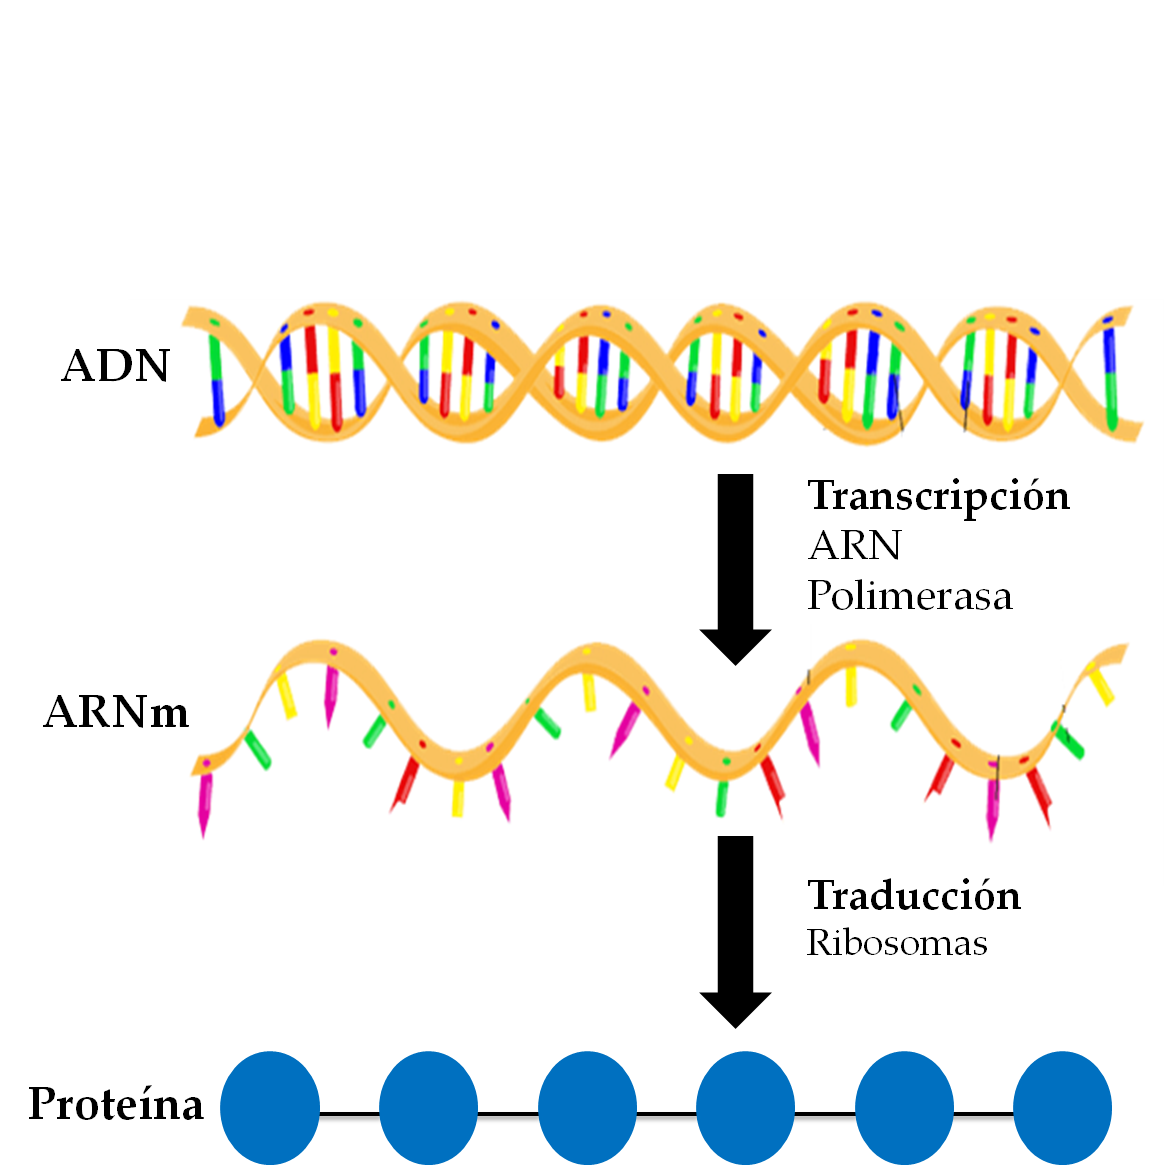
\includegraphics[width=1\textwidth]{Pcon-dogma}
\end{figure}

\column{.5\textwidth}

\begin{figure}[p]
    \centering
    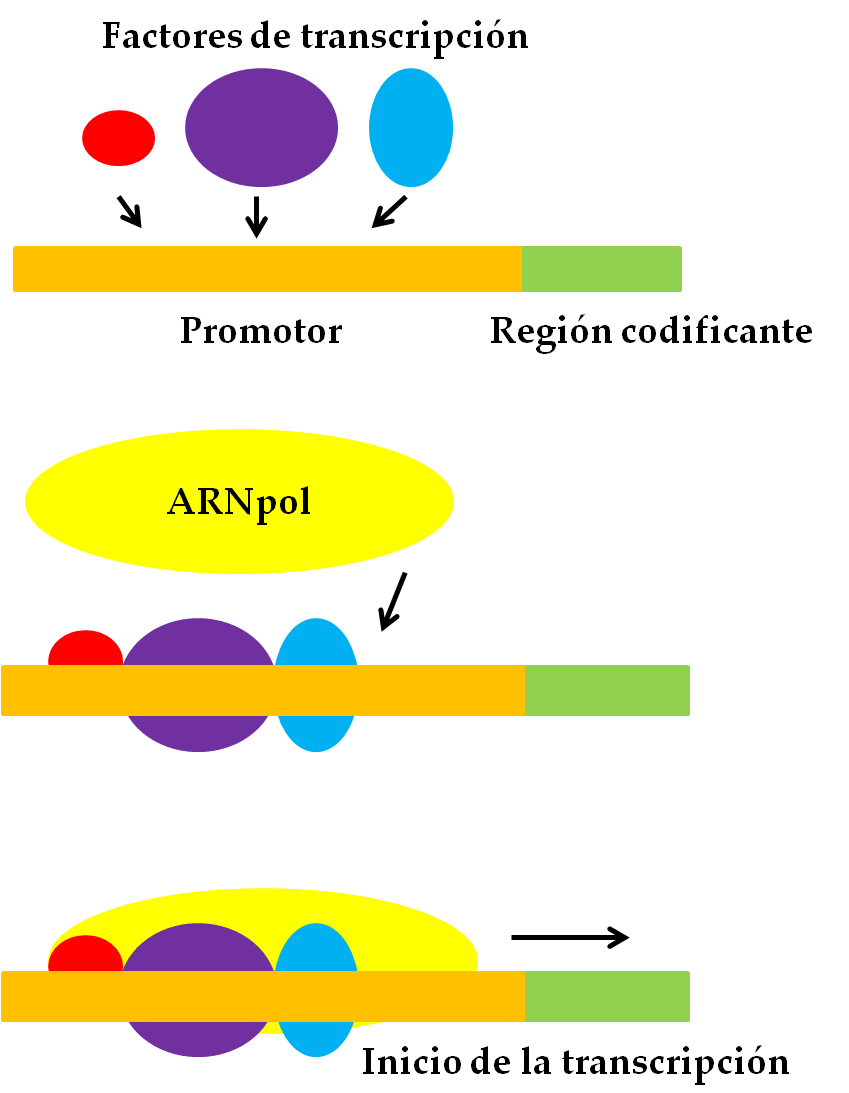
\includegraphics[width=.9\textwidth]{con-tf_simple}
\end{figure}
\end{columns}
\end{frame}

\subsection{Circuitos gen\'eticos}
\begin{frame}
  \begin{figure}[p]
    \centering
    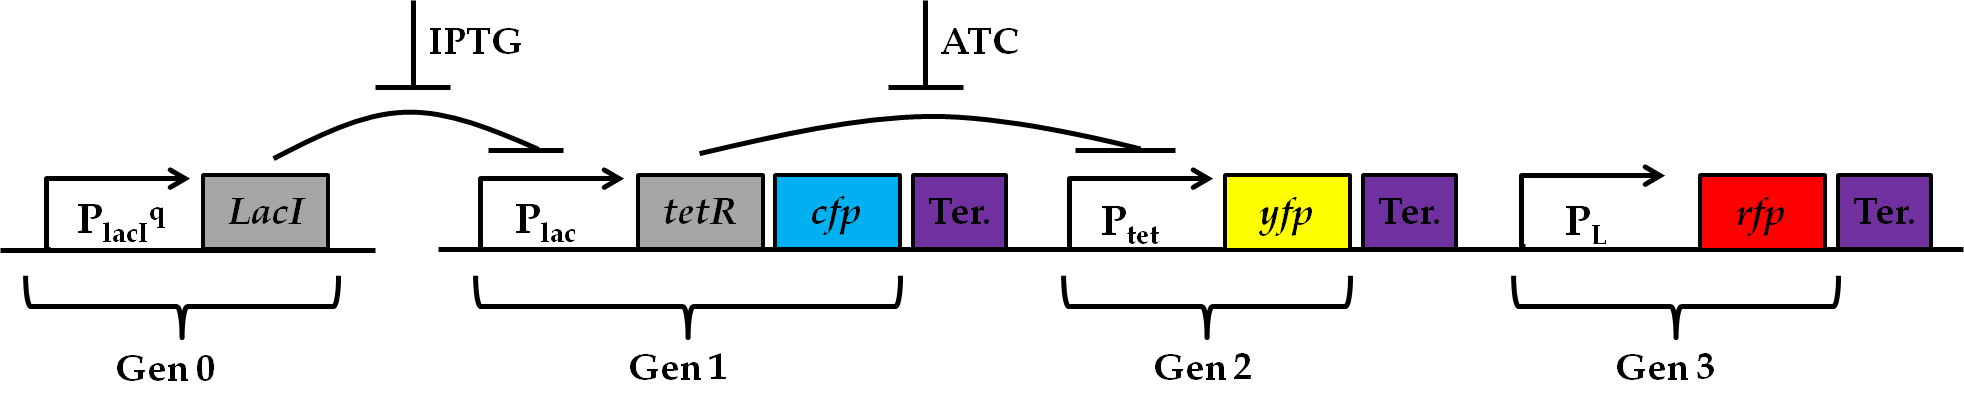
\includegraphics[width=1\textwidth]{Pcon-circuit_simple}~\\
    \tiny Pedraza y van Oudenaarden (2005).
  \end{figure}

\begin{columns}[c]

\column{.3\textwidth}

\begin{figure}[p]
    \centering
    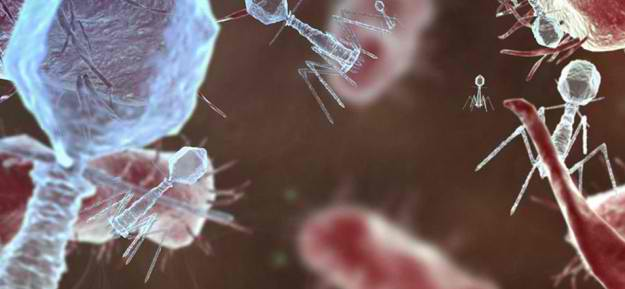
\includegraphics[width=\textwidth]{phageim}~\\
    \tiny Tomado de \url{phages.org}.
\end{figure}

\column{.7\textwidth}
\vspace{-5mm}
\begin{figure}[p]
    \centering
    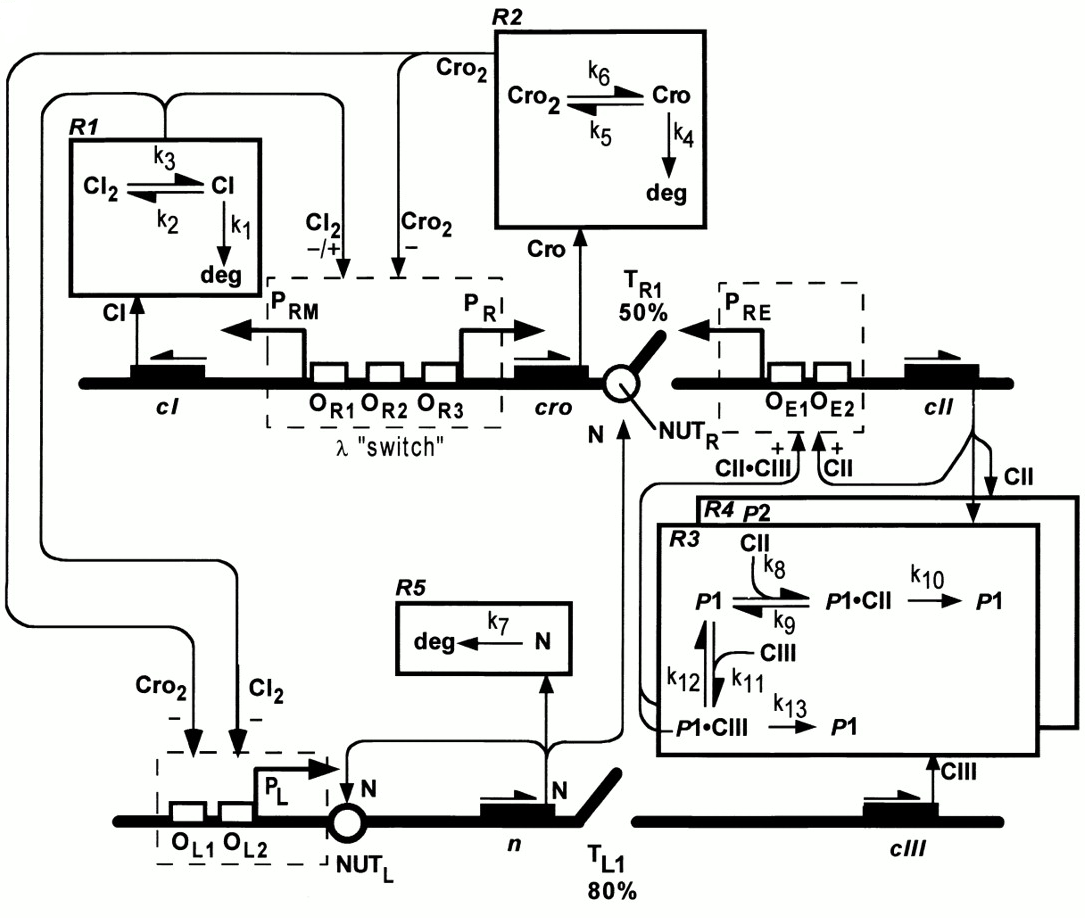
\includegraphics[width=0.6\textwidth]{con-biocircuits_comp.png}~\\
    \tiny Arkin y col. (1998).
\end{figure}
\end{columns}
\end{frame}


\subsection{Ruido en circuitos gen\'eticos}
\begin{frame}
\begin{itemize}
\item Fluctuaciones aleatorias en expresi\'on gen\'etica.
\item En transcripci\'on y traducci\'on: Colisiones aleatorias entre mol\'eculas que se encuentran en bajo n\'umero (Intr\'inseco).

Para \textit{E. coli} en promedio

$$\langle r\rangle_s \approx 5 \text{ ARNs}$$
$$\langle p\rangle_s \approx 3000 \text{ prote\'inas}$$

\item Otros factores como la divisi\'on celular y la variablidad del ambiente (Extr\'inseco).
\begin{align*}
\eta_X &= \frac{\sigma_X}{\langle X \rangle}.\\[1.5ex]
\nu_X &= \frac{\sigma^2_X}{\langle X \rangle}.
\end{align*}
\end{itemize}
\end{frame}

\subsection{Motivaciones para el estudio del ruido}
\begin{frame}

\begin{itemize}
\item Los efectos del ruido son muy notorios.
\end{itemize}

\begin{figure}[p]
    \centering
    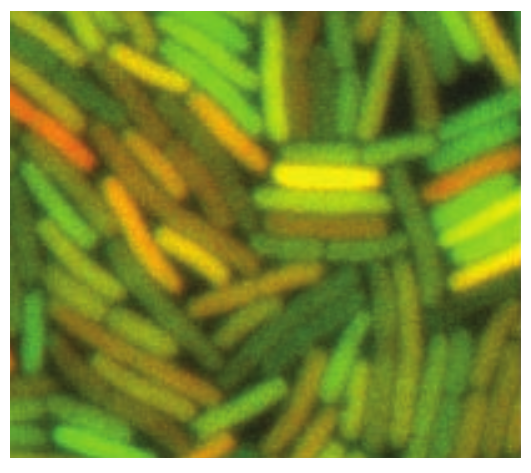
\includegraphics[width=.5\textwidth]{int-noise1}~\\
    \tiny Elowitz y col. (2002).
\end{figure}
\end{frame}

\begin{frame}
\begin{itemize}
\item Estrategias ante el ruido
\end{itemize}

\begin{columns}[c]

\column{.4\textwidth}

\center{Robustez}
\begin{figure}[p]
    \centering
    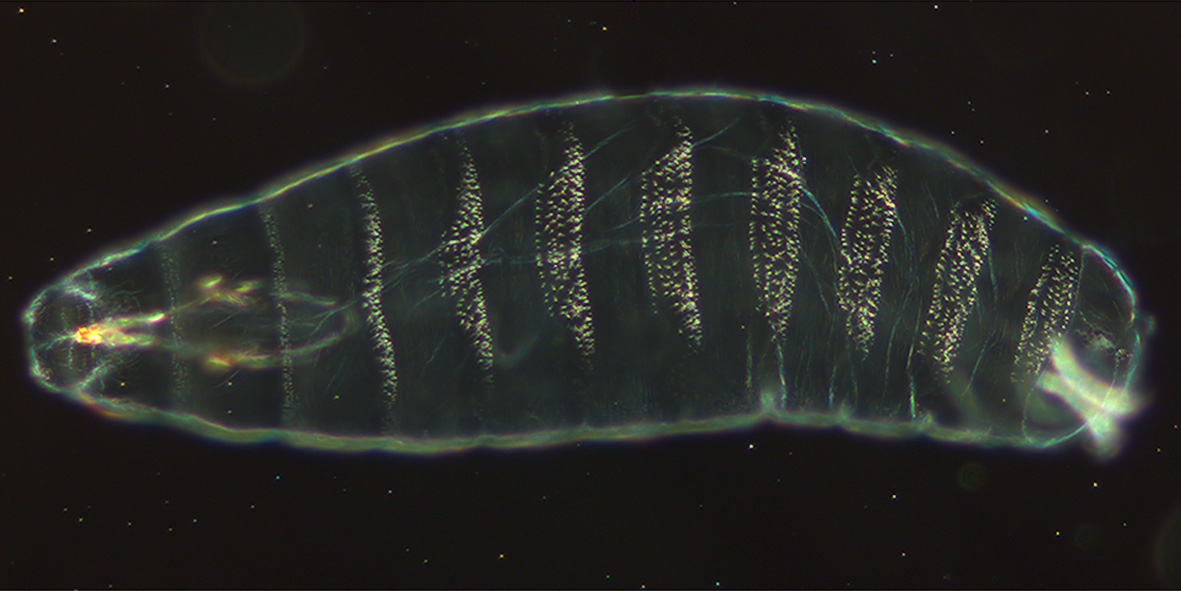
\includegraphics[width=\textwidth]{drosophila}~\\
    \tiny Embri\'on de \textit{D. melanogaster} (mosca de la fruta). Tomado de: \url{https://en.wikipedia.org/wiki/Drosophila_embryogenesis}.
\end{figure}

\column{.6\textwidth}
\center{Variabilidad}

\begin{figure}[p]
    \centering
    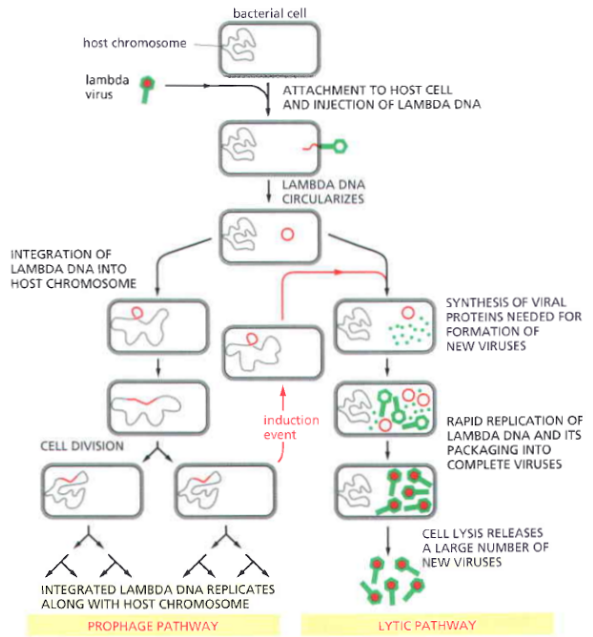
\includegraphics[width=.75\textwidth]{int-lambda}~\\
    \tiny Alberts y col. (2008).
\end{figure}
\end{columns}
\end{frame}

\section{Ecuaci\'on maestra}
\subsection{Gen constitutivo}
\begin{frame}
\begin{columns}[c]
\column{.5\textwidth}
\begin{figure}[p]
    \centering
    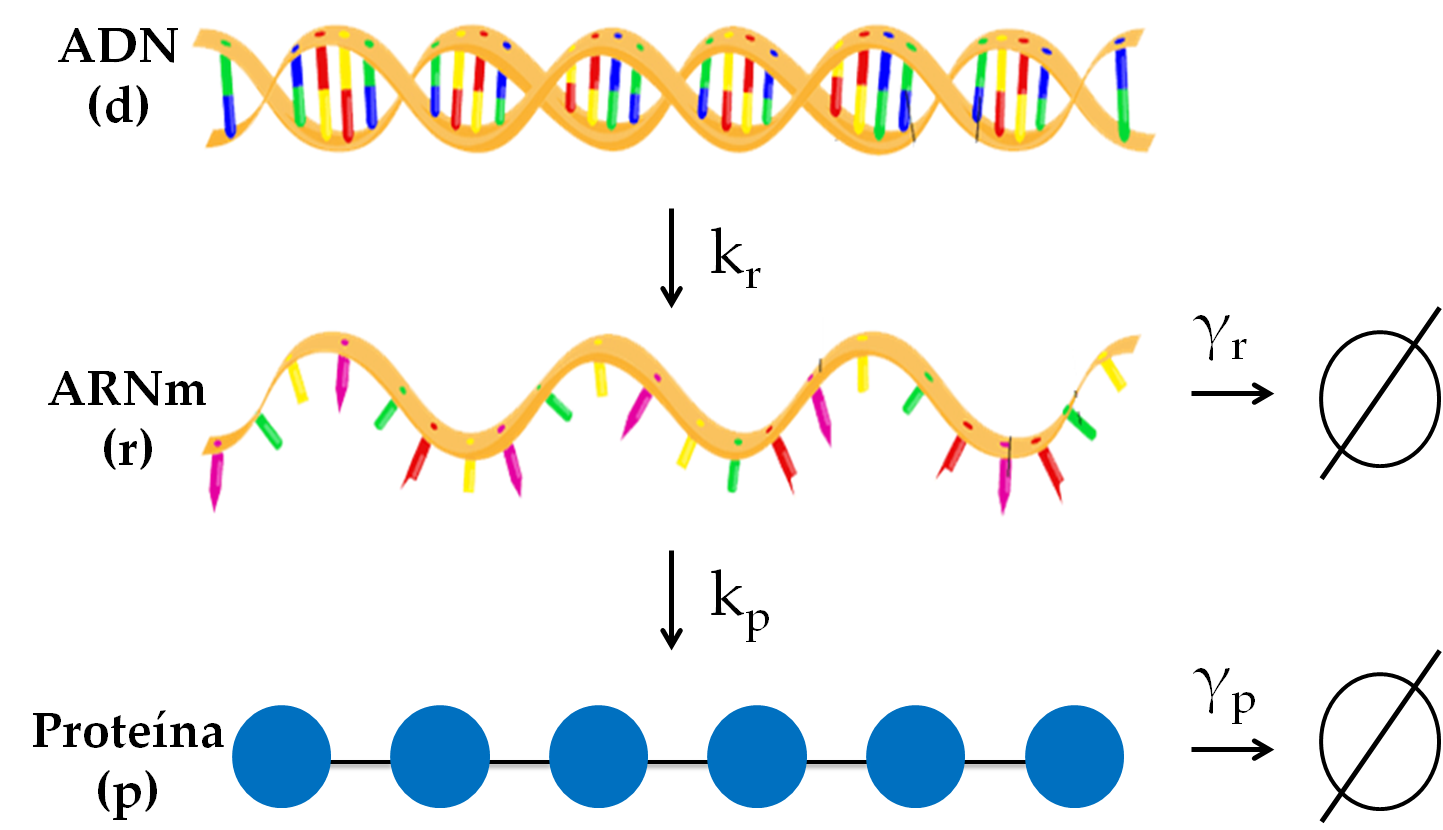
\includegraphics[width=\textwidth]{Pmas-dogma}
\end{figure}
\begin{align*}
\dot{r}(t) &= k_R - \gamma_Rr(t).\\
\dot{p}(t) &= k_Pr(t) - \gamma_Pp(t).
\end{align*}
\column{0.55\textwidth}
\begin{figure}[p]
    \centering
    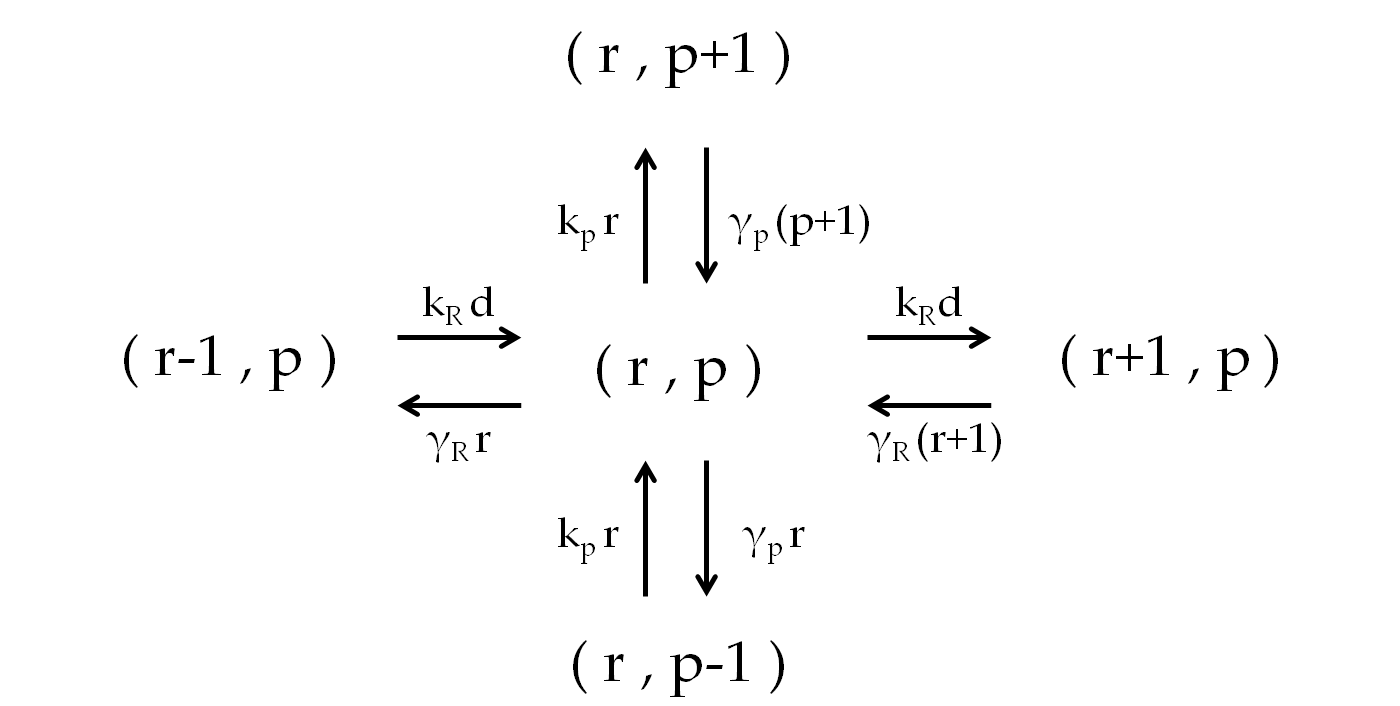
\includegraphics[width=\textwidth]{Pmas-trans_single}
\end{figure}
\begin{align*}
&\frac{d{f}_{r,p}}{dt} = k_Rf_{r-1,p} - k_Rf_{r,p}\\
&+ k_Prf_{r,p-1} - k_Prf_{r,p} + \gamma_R(r+1)f_{r+1,p}\\
&- \gamma_Rrf_{r,p} + \gamma_P(p+1)f_{r,p+1} - \gamma_Ppf_{r,p}.
\end{align*}
\end{columns}
\end{frame}


\begin{frame}

\begin{columns}[c]
\column{.45\textwidth}
\centering \textbf{Promedio}
\begin{align*}
\langle r \rangle &= \frac{k_R}{\gamma_R}.\\[1.5ex]
\langle p \rangle &= \frac{k_Rb}{\gamma_P}.
\end{align*}
\column{.5\textwidth}
\centering \textbf{Ruido}
\begin{align*}
\nu_r &= \frac{\sigma_r^2}{\langle r \rangle} = 1.\\[1.5ex]
\nu_p &= \frac{\sigma_p^2}{\langle p \rangle} = \frac{b}{1+\eta} + 1 \approx b + 1.
\end{align*}
\end{columns}

\vspace{3 mm}

\begin{equation*}
b \coloneqq \frac{k_P}{\gamma_R}, \quad \eta \coloneqq \frac{\gamma_P}{\gamma_R}.
\end{equation*}

\end{frame}

\subsection{Generalizaci\'on del modelo}
\begin{frame}

Las ecuaciones

\begin{align*}
\dot{r}(t) &= k_r - \gamma_rr(t),\\
\dot{p}(t) &= k_pr(t) - \gamma_pp(t),
\end{align*}

pueden ser escritas como

\begin{equation*}
\mathbf{\dot{q}} = (A - \Gamma)\mathbf{q}.
\end{equation*}

Donde $\mathbf{q}^T \coloneqq (d, r, p)$ y

\begin{align*}
A \coloneqq \bordermatrix{
  ~ & (d) & (r) & (p) \cr
  (d) & 0 & 0 & 0 \cr
  (r) & k_R & 0 & 0 \cr
  (p) & 0 & k_P & 0 \cr}, \quad \quad
\Gamma \coloneqq \bordermatrix{
  ~ & (d) & (r) & (p) \cr
  (d) & 0 & 0 & 0 \cr
  (r) & 0 & \gamma_R & 0 \cr
  (p) & 0 & 0 & \gamma_P \cr}.\\
\end{align*}
\end{frame}

\begin{frame}
Se puede realizar en general. Si $\mathbf{q}^T \coloneqq (q_1,q_2,\dots,q_n)$,
la ecuaci\'on maestra queda
\begin{equation*}
\dot{f}= \sum_i\sum_j \left[\left(A_{ij}q_j\right) \left(f_{q_{i-1}} - f_{q_i}\right)\right] + \Gamma_{ii}(q_i+1)f_{q_{i+1}} -\Gamma_{ii}q_if_{q_i}.
\end{equation*}

Al realizar todo el procedimiento obtenemos en estado estacionario

$$\left(\mathbf{A} - \mathbf{\Gamma}\right)\langle \mathbf{q} \rangle = 0.$$

$$0 = \left( \left( \mathbf{\Gamma} - \mathbf{A}\right) \nabla\nabla^TF|_1 - \mathbf{A}\Theta F|_1 \right) +  \left( \left( \mathbf{\Gamma} - \mathbf{A}\right) \nabla\nabla^TF|_1 - \mathbf{A}\Theta F|_1\right)^T,$$ 
$$\Theta_{ij} \coloneqq \delta_{ij}\frac{\partial}{\partial z_i}.$$
\end{frame}


%%%%%%%%%%%%%%%%%%%%%%%%%%%%%%%%%%%%%

\subsection{Autorregulaci\'on}
\begin{frame}
\begin{columns}[c]
\column{.5\textwidth}

\begin{figure}[p]
    \centering
    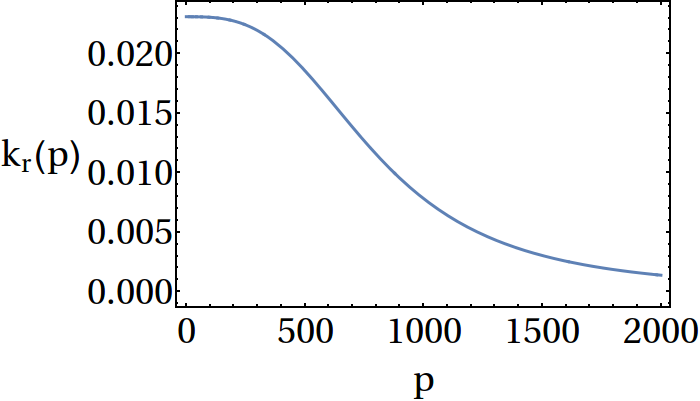
\includegraphics[width=1\textwidth]{Pmas-hill}
\end{figure}
\vspace{-5mm}
\begin{figure}[p]
    \centering
    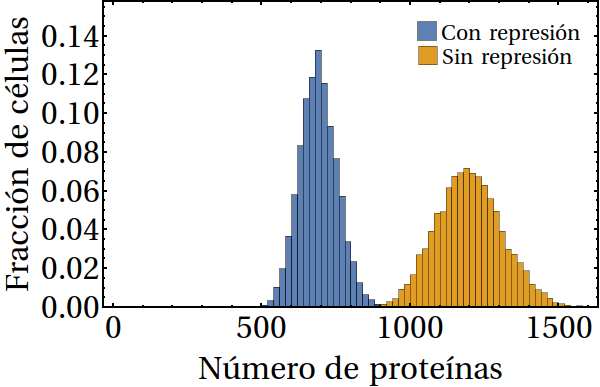
\includegraphics[width=1\textwidth]{Pmas-hist}
\end{figure}

\column{.5\textwidth}

\begin{itemize}

\item Ecuaci\'on de Hill.

\begin{equation*}
k_R = \frac{k_R^{\text{max}}}{1+(p/K_d)^n}.
\end{equation*}

\item Linearizar alrededor del promedio en estado estacionario.

\begin{equation*}
k_R \approx k_0-k_1p.
\end{equation*}

\vspace{-1mm}

\begin{equation*}
A = 
\begin{pmatrix}
0 & 0 & 0 \\
k_0 & 0 & -k_1 \\
0 & k_P & 0
\end{pmatrix}.
\end{equation*}
\end{itemize}
\end{columns}
\end{frame}

%%%%%%%%%%%%%%%%%%%%%%%%%%%%%%%%%%%%%%%
\begin{frame}
\begin{columns}[c]

\vspace{3mm}

\column{.45\textwidth}

\centering \textbf{Promedio}
\begin{align*}
%\langle r \rangle &= .\\[1.5ex]
\langle p \rangle &= \frac{1}{1+b\phi} \cdot \frac{k_0b}{\gamma_p}.
\end{align*}

\column{.5\textwidth}
\centering \textbf{Ruido}
\begin{align*}
%\nu_r &= .\\[1.5ex]
\nu_p &= \frac{1-\phi}{1+b\phi} \cdot \frac{b}{1+\eta}+1.
\end{align*}
\end{columns}

\vspace{3 mm}

\begin{equation*}
  b \coloneqq \frac{k_P}{\gamma_R}, \quad \eta \coloneqq \frac{\gamma_P}{\gamma_R}, \quad \phi \coloneqq \frac{k_1}{\gamma_P}.
\end{equation*}

\begin{figure}[p]
    \centering
    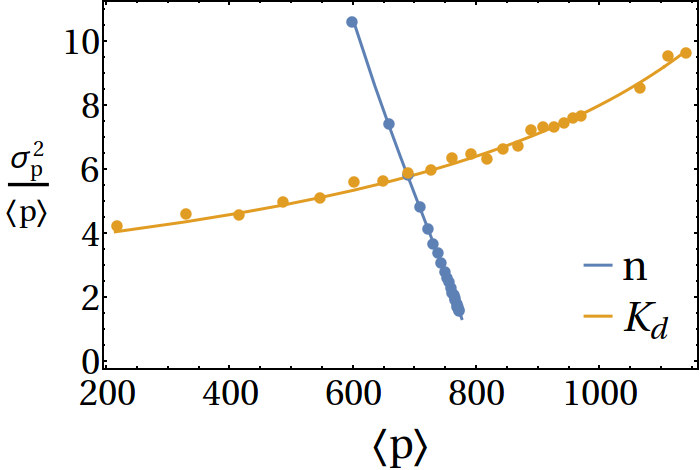
\includegraphics[width=0.5\textwidth]{Pmas-autorreg_analytic_solver}
\end{figure}

\end{frame}

\section{Ecuaci\'on de Langevin}

\begin{frame}
\begin{figure}[p]
    \centering
    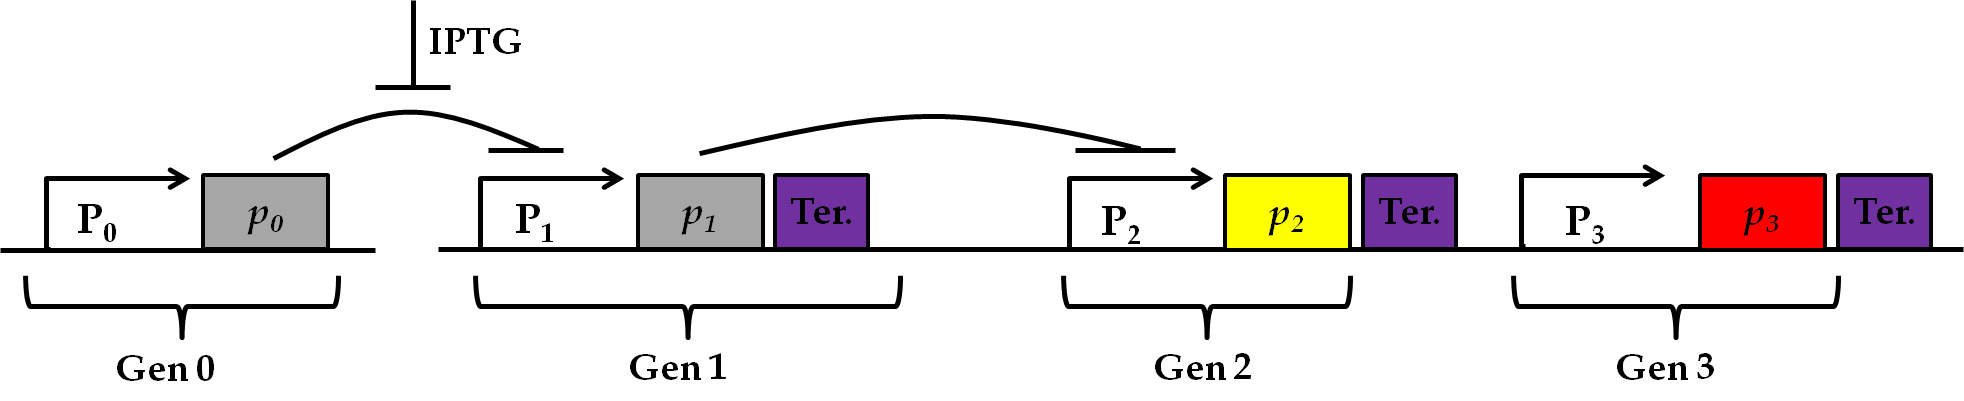
\includegraphics[width=\textwidth]{lan-Circuit}\\
    \tiny Pedraza y van Oudenaarden (2005).
\end{figure}
\end{frame}

\subsection{Ec. de Langevin - Gen 0}
\begin{frame}
Ecuaci\'on determinista con t\'erminos de ruido. Para el gen 0
$$\dot{p_0} = k - \gamma p_0 + \mu_0 + \xi_{0}.$$
Los t\'erminos de ruido cumplen:
$$\langle \mu_0 \rangle = \langle \xi_0 \rangle = 0,$$
$$\langle \mu_0(t)\mu_0(t+\tau) \rangle  = 2\gamma (b_0+1) \bar{p_0} \delta(\tau),$$
$$\langle \xi_0(t)\xi_0(t+\tau) \rangle = 2 \gamma \eta_{_G}^2\bar{p_0}^2 \delta(\tau),$$
$$\langle \mu_0(t)\xi_0(t+\tau) \rangle = 0.$$
Luego de hacer el proceso:
$$\eta_0^2=\frac{b_0+1}{\bar{p_0}} + \eta_{G}^2\coloneqq\eta_{0\,\text{int}}^2+\eta_{G}^2$$
\end{frame}

\subsection{Ec. de Langevin - Gen 1}
\begin{frame}
Ahora para el gen 1
$$\dot{p_1} = f_1(p_{0,\text{disp}}) - \gamma p_1 + \mu_1 + \xi_1$$
Adem\'as de las anteriores autocorrelaciones, hay que incluir:
$$\langle \xi_0(t)\xi_1(t+\tau) \rangle = 2 \gamma \eta_{_G}^2\bar{p_0}\bar{p_1}\delta(\tau),$$
$$\langle \mu_0(t)\mu_1(t+\tau) \rangle =0.$$
Se obtiene al final
$$\eta_1^2 = \eta_{1\,\text{int}}^2 + \frac{1}{2} H_{10}^2 \eta_{0\,\text{int}}^2 + \eta_G^2\left( 1 + \frac{1}{2} H_{10}^2 - H_{10} \right)$$
\end{frame}

\subsection{Distintas fuentes de ruido y su propagaci\'on}
\begin{frame}
\begin{figure}[p]
    \centering
    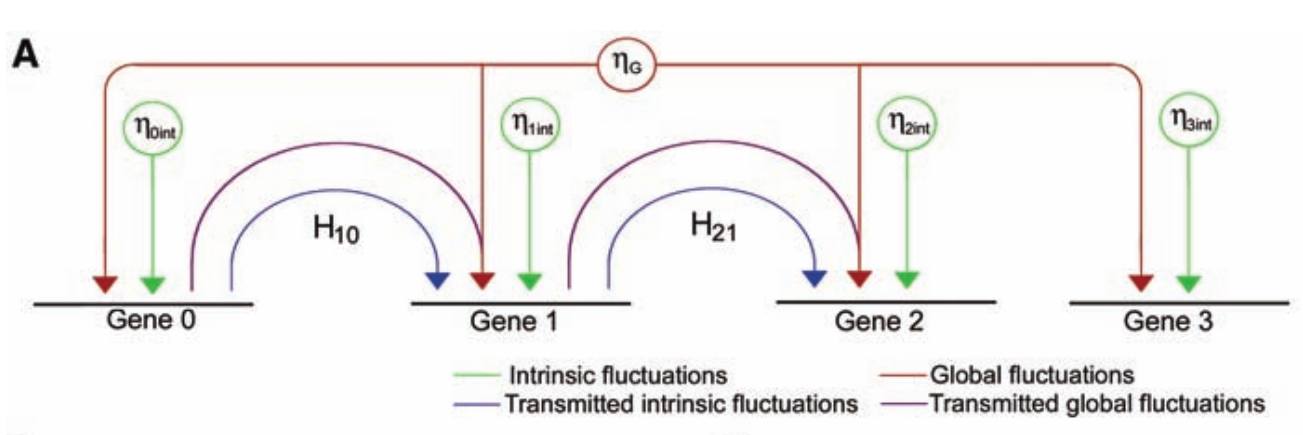
\includegraphics[width=\textwidth]{globalint.png}\\
    \tiny Pedraza y van Oudenaarden (2005).
\end{figure}
\end{frame}

%Muy chevere porque no se saben con precision las fuentes del ruido global pero a partir de sus estadisticas se puede hallar el ruido

\subsection{Ganancia logar\'itmica}
\begin{frame}
\begin{figure}[p]
    \centering
    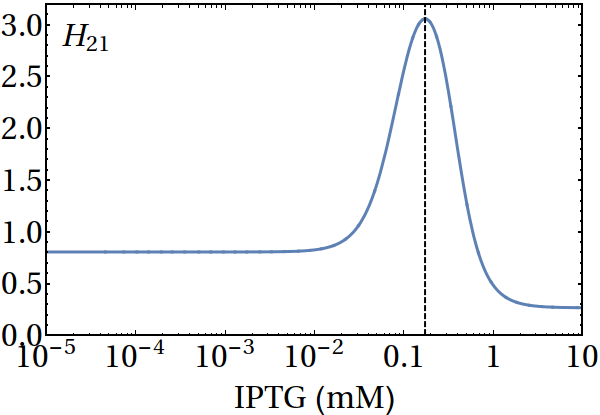
\includegraphics[width=.7\textwidth]{lan-H21.png}\\
\end{figure}
\end{frame}

\subsection{Ruidos y correlaciones}
\begin{frame}
\vspace{-4mm}
\begin{columns}[c]
\column{.5\textwidth}

\begin{figure}[p]
    \centering
    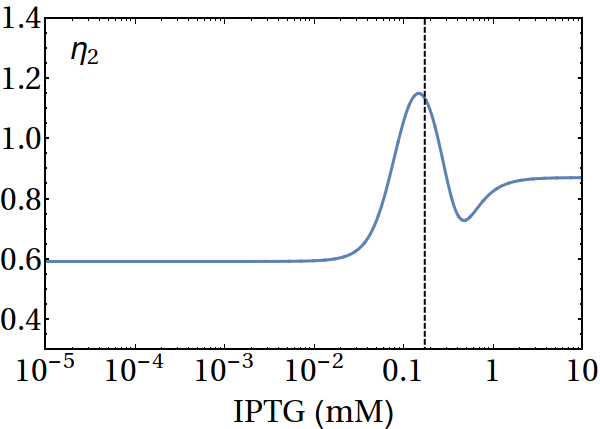
\includegraphics[width=\textwidth]{lan-eta2.png}
\end{figure}
\column{.5\textwidth}

\begin{figure}[p]
    \centering
    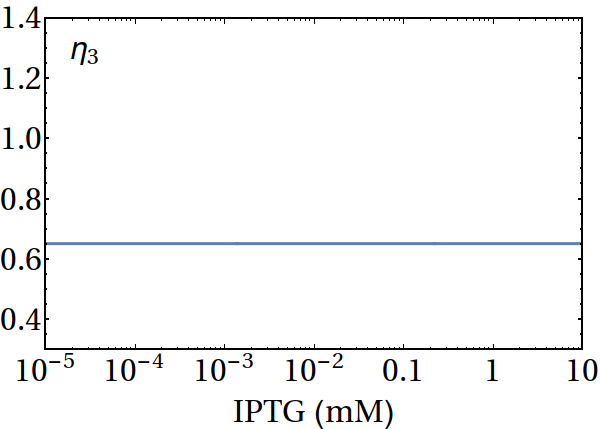
\includegraphics[width=\textwidth]{lan-eta3.png}
\end{figure}
\end{columns}
\begin{figure}[p]
    \centering
    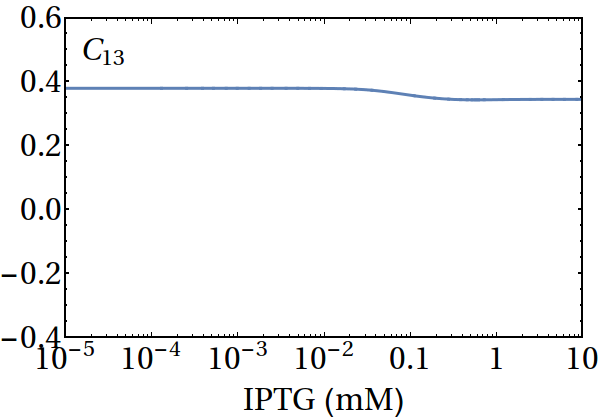
\includegraphics[width=.5\textwidth]{lan-c13.png}\\
\end{figure}
\end{frame}

\section{Divisi\'on celular}

\subsection{Segregaci\'on ordenada y desordenada}
\begin{frame}
\begin{figure}[p]
    \centering
    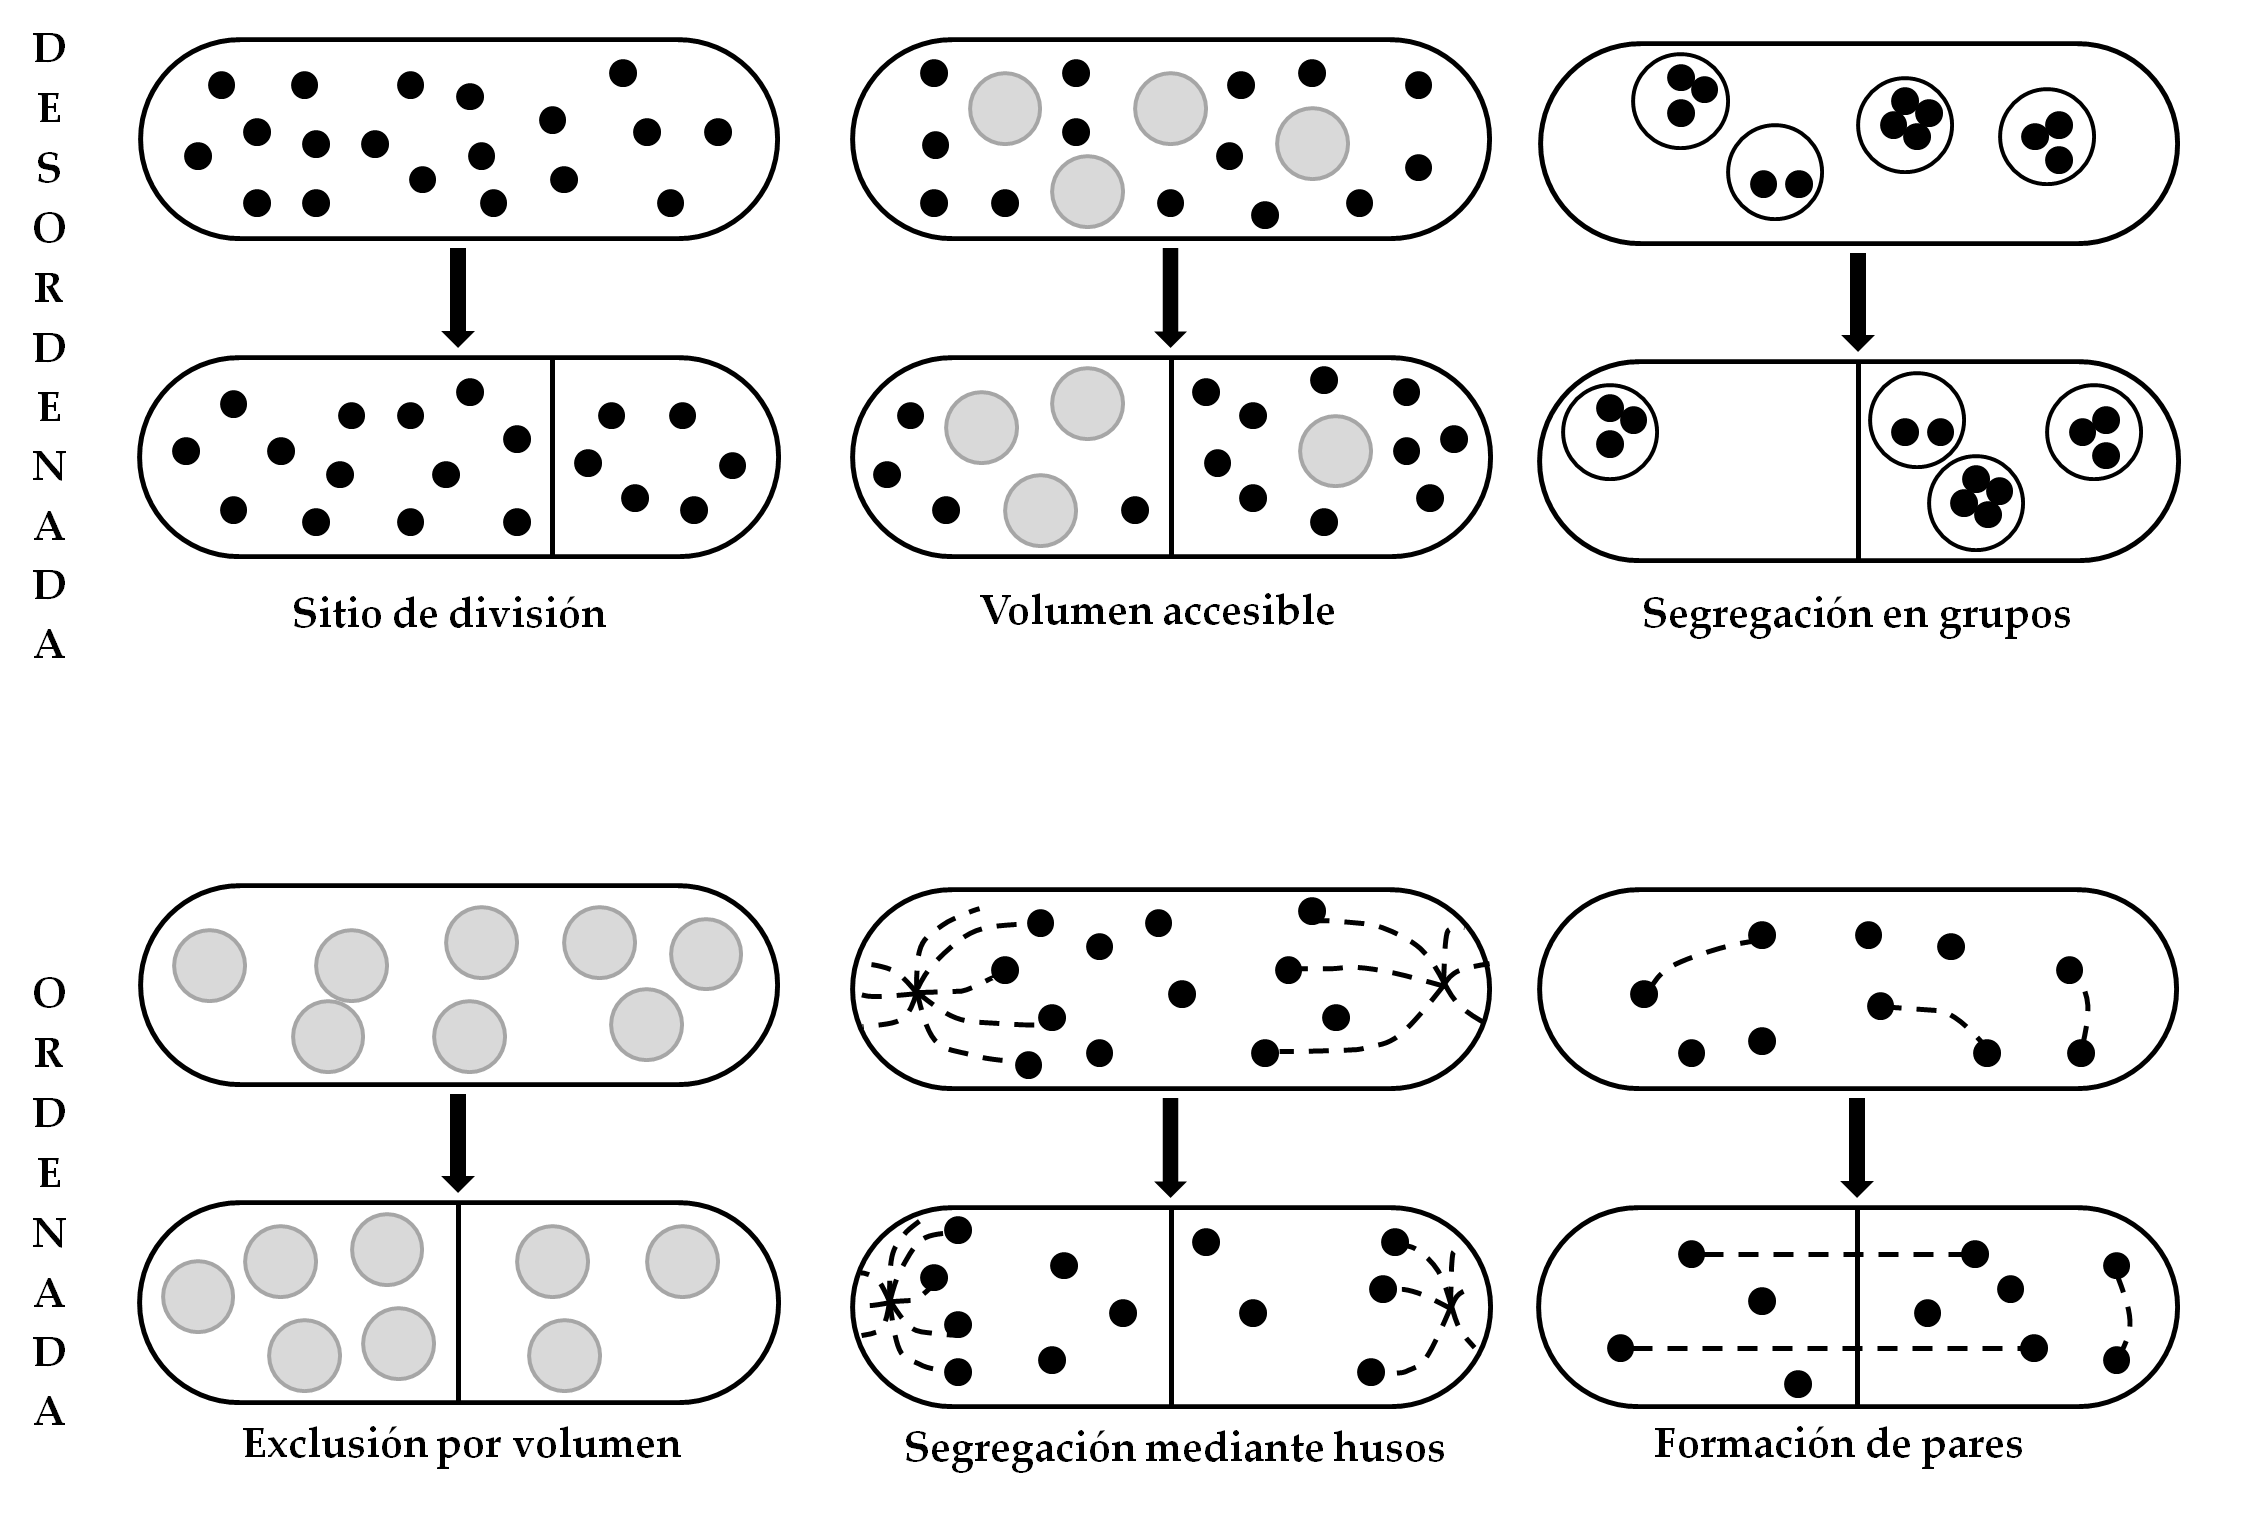
\includegraphics[width=\textwidth]{Pdiv-draws}
\end{figure}
\end{frame}

\subsection{Ruido por partici\'on}
\begin{frame}

Para un componente $X$, donde $L$ y $R$ copias se segregan a cada hija, el error en la partici\'on est\'a dado por

$$Q_X^2 = \frac{\langle (L-R)^2 \rangle}{\langle X \rangle^2}. $$

Para segregaci\'on independiente:

$$Q_X = \frac{1}{\sqrt{X}}.$$

Para los mecanismos considerados

$$ Q_X^2 = \frac{A}{X}, \quad \text{donde} \quad 
\begin{cases}
A = 1 \quad \text{para segregaci\'on independiente,}\\
A < 1 \quad \text{para segregaci\'on ordenada,}\\
A > 1 \quad \text{para segregaci\'on desordenada.}
\end{cases} 
$$
%De nuevo problema con los ajustes.

\end{frame}

%%%%%%%%%%%%%%%%%%%%%%%%%%%%%%%%

\section{Conclusiones}
\subsection{Conclusiones}
\begin{frame}
\begin{itemize}
\item Ecuaci\'on maestra vs. ecuaci\'on de Langevin.
\item Dificultad para identificar las fuentes de ruido.
\item T\'ecnicas experimentales para medir con mayor resoluci\'on.
\end{itemize}
\end{frame}
\subsection{Trabajo futuro}
\begin{frame}
\begin{itemize}

\item Analizar el ruido por partici\'on mediante simulaciones que lo integren con transcripci\'on y traducci\'on.
\item Analizar la aleatoriedad en el volumen de la c\'elula.

\end{itemize}
\end{frame}

\begin{frame}[allowframebreaks]
\printbibliography
\end{frame}

\end{document}
